\documentclass[tikz,border=2mm]{standalone}
\begin{document}
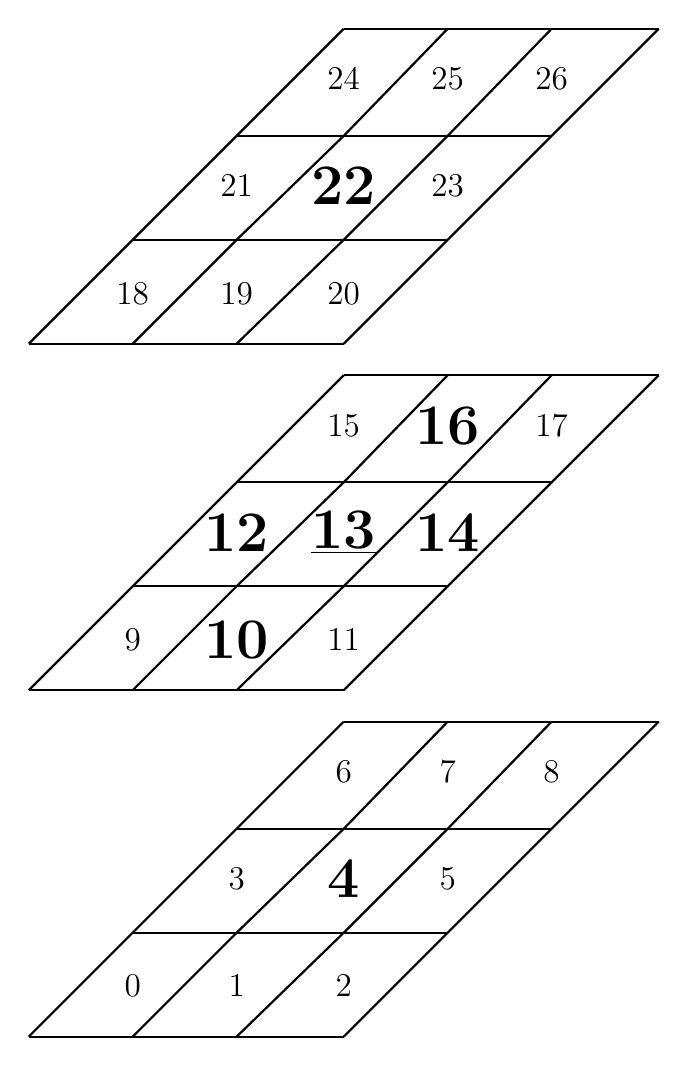
\begin{tikzpicture}[scale=4,thick]
%%%%%%%%%%%%%%%%%%%%%%%%%%%%%%%%
%% iz=0 layer
%%%%%%%%%%%%%%%%%%%%%%%%%%%%%%%%
\draw[-] (0,0)   --(0.33,0.33);
\draw[-] (0.33,0)--(0.66,0.33);
\draw[-] (0.66,0)--(1,0.33);
\draw[-] (1,0)   --(1.33,0.33);

\draw[-] (0.33,0.33)--(0.66,0.66);
\draw[-] (0.66,0.33)--(1,0.66);
\draw[-] (1,0.33)--(1.33,0.66);
\draw[-] (1.33,0.33)--(1.66,0.66);

\draw[-] (0.66,0.66)--(1,1);
\draw[-] (1.33,0.66)--(1.66,1);
\draw[-] (1,0.66)--(1.33,1);
\draw[-] (1.66,0.66)--(2,1);
%
\draw[-] (0,0)--(0.33,0);
\draw[-] (0.33,0)--(0.66,0);
\draw[-] (0.66,0)--(1,0);

\draw[-] (0.33,0.33)--(0.66,0.33);
\draw[-] (0.66,0.33)--(1,0.33);
\draw[-] (1,0.33)--(1.33,0.33);

\draw[-] (0.66,0.66)--(1,0.66);
\draw[-] (1,0.66)--(1.33,0.66);
\draw[-] (1.33,0.66)--(1.66,0.66);

\draw[-] (1,1)--(1.33,1);
\draw[-] (1.33,1)--(1.66,1);
\draw[-] (1.66,1)--(2,1);

\large
\draw (0.33,0.16) node {0};
\draw (0.66,0.16) node {1};
\draw (1,0.16) node {2};
\draw (0.66,0.5) node {3};
\huge
\draw (1,0.5) node {\textbf{4}};
\large
\draw (1.33,0.5) node {5};
\draw (1,0.84) node {6};
\draw (1.33,0.84) node {7};
\draw (1.66,0.84) node {8};


%%%%%%%%%%%%%%%%%%%%%%%%%%%%%%%%
%% iz=1 layer
%%%%%%%%%%%%%%%%%%%%%%%%%%%%%%%%
\draw[-] (0,0+1.10)   --(0.33,0.33+1.10);
\draw[-] (0.33,0+1.10)--(0.66,0.33+1.10);
\draw[-] (0.66,0+1.10)--(1,0.33+1.10);
\draw[-] (1,0+1.10)   --(1.33,0.33+1.10);

\draw[-] (0.33,0.33+1.10)--(0.66,0.66+1.10);
\draw[-] (0.66,0.33+1.10)--(1,0.66+1.10);
\draw[-] (1,0.33+1.10)--(1.33,0.66+1.10);
\draw[-] (1.33,0.33+1.10)--(1.66,0.66+1.10);

\draw[-] (0.66,0.66+1.10)--(1,1+1.10);
\draw[-] (1.33,0.66+1.10)--(1.66,1+1.10);
\draw[-] (1,0.66+1.10)--(1.33,1+1.10);
\draw[-] (1.66,0.66+1.10)--(2,1+1.10);
%
\draw[-] (0,0+1.10)--(0.33,0+1.10);
\draw[-] (0.33,0+1.10)--(0.66,0+1.10);
\draw[-] (0.66,0+1.10)--(1,0+1.10);

\draw[-] (0.33,0.33+1.10)--(0.66,0.33+1.10);
\draw[-] (0.66,0.33+1.10)--(1,0.33+1.10);
\draw[-] (1,0.33+1.10)--(1.33,0.33+1.10);

\draw[-] (0.66,0.66+1.10)--(1,0.66+1.10);
\draw[-] (1,0.66+1.10)--(1.33,0.66+1.10);
\draw[-] (1.33,0.66+1.10)--(1.66,0.66+1.10);

\draw[-] (1,1+1.10)--(1.33,1+1.10);
\draw[-] (1.33,1+1.10)--(1.66,1+1.10);
\draw[-] (1.66,1+1.10)--(2,1+1.10);

\large
\draw (0.33,0.16+1.10) node {9};
\huge
\draw (0.66,0.16+1.10) node {\textbf{10}};
\large
\draw (1,0.16+1.10) node {11};
\huge
\draw (0.66,0.5+1.10) node {\textbf{12}};
\draw (1,0.5+1.10) node {\underline{\textbf{13}}};
\draw (1.33,0.5+1.10) node {\textbf{14}};
\large
\draw (1,0.84+1.10) node {15};
\huge
\draw (1.33,0.84+1.10) node {\textbf{16}};
\large
\draw (1.66,0.84+1.10) node {17};
%%%%%%%%%%%%%%%%%%%%%%%%%%%%%%%%
%% iz=2 layer
%%%%%%%%%%%%%%%%%%%%%%%%%%%%%%%%
\draw[-] (0,0+2.20)   --(0.33,0.33+2.20);
\draw[-] (0.33,0+2.20)--(0.66,0.33+2.20);
\draw[-] (0.66,0+2.20)--(1,0.33+2.20);
\draw[-] (1,0+2.20)   --(1.33,0.33+2.20);

\draw[-] (0.33,0.33+2.20)--(0.66,0.66+2.20);
\draw[-] (0.66,0.33+2.20)--(1,0.66+2.20);
\draw[-] (1,0.33+2.20)--(1.33,0.66+2.20);
\draw[-] (1.33,0.33+2.20)--(1.66,0.66+2.20);

\draw[-] (0.66,0.66+2.20)--(1,1+2.20);
\draw[-] (1.33,0.66+2.20)--(1.66,1+2.20);
\draw[-] (1,0.66+2.20)--(1.33,1+2.20);
\draw[-] (1.66,0.66+2.20)--(2,1+2.20);
%
\draw[-] (0,0+2.20)--(0.33,0+2.20);
\draw[-] (0.33,0+2.20)--(0.66,0+2.20);
\draw[-] (0.66,0+2.20)--(1,0+2.20);

\draw[-] (0.33,0.33+2.20)--(0.66,0.33+2.20);
\draw[-] (0.66,0.33+2.20)--(1,0.33+2.20);
\draw[-] (1,0.33+2.20)--(1.33,0.33+2.20);

\draw[-] (0.66,0.66+2.20)--(1,0.66+2.20);
\draw[-] (1,0.66+2.20)--(1.33,0.66+2.20);
\draw[-] (1.33,0.66+2.20)--(1.66,0.66+2.20);

\draw[-] (1,1+2.20)--(1.33,1+2.20);
\draw[-] (1.33,1+2.20)--(1.66,1+2.20);
\draw[-] (1.66,1+2.20)--(2,1+2.20);

\large
\draw (0.33,0.16+2.20) node {18};
\draw (0.66,0.16+2.20) node {19};
\draw (1,0.16+2.20) node {20};
\draw (0.66,0.5+2.20) node {21};
\huge
\draw (1,0.5+2.20) node {\textbf{22}};
\large
\draw (1.33,0.5+2.20) node {23};
\draw (1,0.84+2.20) node {24};
\draw (1.33,0.84+2.20) node {25};
\draw (1.66,0.84+2.20) node {26};
\end{tikzpicture}
\end{document}
